\usetikzlibrary{arrows,calc,fit,matrix,positioning}
\definecolor{coral}{RGB}{255,127,80}
\definecolor{ma}{RGB}{102,205,170}
\definecolor{dsb}{RGB}{0,191,255}

\newcommand{\CC}{C++}
\defcitealias{posix7}{POSIX~7, 2018}
\defcitealias{openmp08}{OpenMP~v.3, 2008}

Cross-validation is the gold standard for evaluating machine learning
algorithms or fine-tuning their parameters.
The results of this technique, however, are not always reproducible and may
depend on the computing platform and the number of parallel threads,
especially if the underlying learning algorithm uses a pseudo-random number
generator~(PRNG). This paper gives a recipe for solving these reproducibility problems and
applies it to LIBLINEAR\supercite{fan2008liblinear}, a popular software library
that implements randomized learning algorithms based on support vector
machines\supercite{vapnik1998statistical}. The proposed approach solves these
problems by using a cross-platform PRNG and by making the PRNG state private
in each thread. The cross-validation results obtained with the modified
version of LIBLINEAR were the same across platforms. Furthermore, the
parallelized cross-validation results were no longer affected by random
fluctuations arising from the sharing of the PRNG state by parallel threads.


\section{Introduction}


The reproducibility of machine learning results has been questioned in the top
scientific journals~\supercite{%
  barnes2010publish,
  peng2011reproducible,
  ince2012case,
  hutson2018artificial}. Similar issues have been brought up in the
Artificial~Intelligence~\supercite{henderson2017deep,gundersen2018state} and
Machine~Learning~\supercite{sculley2015hidden} communities.
According to~\citet{henderson2017deep}, reproducibility problems can be
\emph{extrinsic}, i.e., unrelated to the algorithms or their implementations,
or \emph{intrinsic}, i.e., directly associated with the algorithms, their
implementations, or the computing environments in which they run. This paper
describes a technique that eliminates two intrinsic problems that may impede
the reproducibility of cross-validation results for randomized learning algorithms.
The first problem stems from using a platform-dependent pseudo-random number
generator~(PRNG). The second problem is due to sharing the PRNG state by
parallel threads.

\smallskip
Cross-validation (CV) is a statistical technique 
that is often used to evaluate machine learning algorithms or to select their
parameters (see Figure~\ref{fig:CV}). It assigns data instances into $N$ folds and then picks $K$ folds
for testing and $N - K$ folds for training. This process is repeated $R$ times and the
results are averaged. Typically, $K=1$ and $R=N$.
Because a PRNG is often used to assign instances to folds, the results may
depend on the platform (i.e., OS, programming language, compiler,
runtime libraries, etc.).
It is straightforward to parallelize CV by distributing the $R$ repetitions over
$T$ threads, but the results can be affected by PRNG state sharing. In
particular, this is true for algorithms implemented in C~or~\CC{} that use the
standard function \verb|rand()|. Furthermore, \verb|rand()| may not even be
thread-safe~\citepalias[\mbox{,} p.~1767]{posix7}.


\begin{figure}
  \centering
  \tikzstyle{block} = [minimum size=1em, outer sep=0pt,inner sep=0,line
             width=0.5pt,append after command={\pgfextra{\draw
             ($(\tikzlastnode.north west)+(-0.2em,+0.2em)$)
             rectangle ($(\tikzlastnode.south east)+(0.2em,-0.2em)$);}}]
  \tikzstyle{greenblock} = [minimum size=1em, outer sep=0pt,inner sep=0,line
  width=0.5pt,fill=ma,
  append after command={\pgfextra{
      \filldraw [fill=ma,draw=black]
      ($(\tikzlastnode.north west)+(-0.15em,+0.15em)$)
      rectangle ($(\tikzlastnode.south east)+(0.15em,-0.15em)$);}}]
  \tikzstyle{redblock} = [minimum size=1em, outer sep=0pt,inner sep=0,line
  width=0.5pt,fill=coral,
  append after command={\pgfextra{
      \filldraw [fill=coral,draw=black]
      ($(\tikzlastnode.north west)+(-0.15em,+0.15em)$)
      rectangle ($(\tikzlastnode.south east)+(0.15em,-0.15em)$);}}]
  \tikzstyle{blueblock} = [minimum size=1em, outer sep=0pt,inner sep=0,line
  width=0.5pt,fill=dsb,
  append after command={\pgfextra{
      \filldraw [fill=dsb,draw=black]
      ($(\tikzlastnode.north west)+(-0.15em,+0.15em)$)
      rectangle ($(\tikzlastnode.south east)+(0.15em,-0.15em)$);}}]
  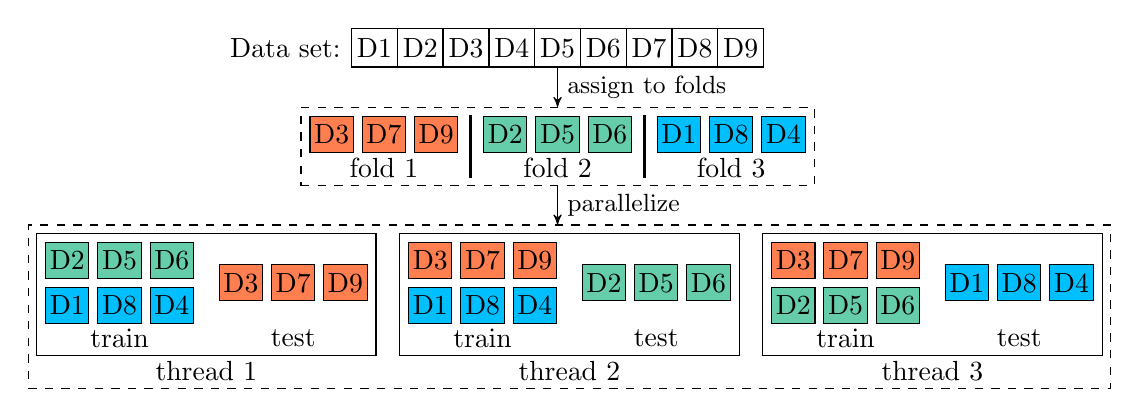
\begin{tikzpicture}[>=stealth']
    \matrix[matrix of nodes, inner sep=0mm,
             nodes=block,
             nodes in empty cells,column sep=-0.5pt, row sep=-0.5pt] (ds) {
      D1 & D2 & D3 & D4 & D5 & D6 & D7 & D8 & D9 \\
    };
    \node[left = 0mm of ds]{Data set:};

    \matrix[below = 6mm of ds, column sep=1mm, inner sep=0mm] (f2) {
      \node[greenblock]{D2}; & \node[greenblock]{D5}; & \node[greenblock]{D6}; \\
    };
    \node[below = 0.5mm of f2, inner sep=0mm] (f2c) {fold 2};

    \matrix[left = 3mm of f2, column sep=1mm, inner sep=0mm] (f1) {
      \node[redblock]{D3}; & \node[redblock]{D7}; & \node[redblock]{D9}; \\
    };
    \node[below = 0.5mm of f1, inner sep=0mm] (f1c) {fold 1};

    \matrix[right = 3mm of f2, column sep=1mm, inner sep=0mm] (f3) {
      \node[blueblock]{D1}; & \node[blueblock]{D8}; & \node[blueblock]{D4}; \\
    };
    \node[below = 0.5mm of f3, inner sep=0mm] (f3c) {fold 3};

    \node[fit=(f1) (f2) (f3) (f1c) (f2c) (f3c), draw, inner sep=1mm,
    draw, dashed] (folds) {};


    \draw[thin, ->] (ds) -- (folds) node[midway,right,font=\small]
    {assign to folds};

    \node at ($(f1.east)!0.5!(f2.west)$) (f12anchor) {};
    \node at ($(f2.east)!0.5!(f3.west)$) (f23anchor) {};

    \draw[very thick] (f12anchor |- f1.north) -- (f12anchor |- f1c.south);
    \draw[very thick] (f23anchor |- f3.north) -- (f23anchor |- f3c.south);


    \matrix[below = 7mm of folds, anchor=north east,
    column sep = 1mm, row sep=1mm, inner sep=0mm] (t2train) {
      \node[redblock]{D3}; & \node[redblock]{D7}; & \node[redblock]{D9}; \\
      \node[blueblock]{D1}; & \node[blueblock]{D8}; & \node[blueblock]{D4}; \\
    };
    \matrix[right = 3mm of t2train, column sep = 1mm, inner sep = 0mm] (t2test) {
      \node[greenblock]{D2}; & \node[greenblock]{D5}; & \node[greenblock]{D6}; \\
    };
    \node[below = 0.5mm of t2train, inner sep=0mm] (t2traincap) {train};
    \node[inner sep=0mm] at (t2traincap -| t2test) (t2testcap) {test};

    \node[fit=(t2train) (t2traincap) (t2test) (t2testcap), draw, inner sep=1mm]
    (t2box) {};
    \node[below = 0.5mm of t2box, inner sep=0mm] {thread 2};


    \matrix[left = 5mm of t2train, column sep = 1mm, inner sep = 0mm] (t1test) {
      \node[redblock]{D3}; & \node[redblock]{D7}; & \node[redblock]{D9}; \\
    };
    \matrix[left = 3mm of t1test, column sep = 1mm, row sep = 1mm,
    inner sep = 0mm] (t1train) {
      \node[greenblock]{D2}; & \node[greenblock]{D5}; & \node[greenblock]{D6}; \\
      \node[blueblock]{D1}; & \node[blueblock]{D8}; & \node[blueblock]{D4}; \\
    };
    \node[below = 0.5mm of t1train, inner sep=0mm] (t1traincap) {train};
    \node[inner sep=0mm] at (t1traincap -| t1test) (t1testcap) {test};

    \node[fit=(t1train) (t1traincap) (t1test) (t1testcap), draw, inner sep=1mm]
    (t1box) {};
    \node[below = 0.5mm of t1box, inner sep=0mm] {thread 1};


    \matrix[right = 5mm of t2test, column sep = 1mm, row sep = 1mm,
    inner sep = 0mm] (t3train) {
      \node[redblock]{D3}; & \node[redblock]{D7}; & \node[redblock]{D9}; \\
      \node[greenblock]{D2}; & \node[greenblock]{D5}; & \node[greenblock]{D6}; \\
    };
    \matrix[right = 3mm of t3train, column sep = 1mm, inner sep = 0mm] (t3test) {
      \node[blueblock]{D1}; & \node[blueblock]{D8}; & \node[blueblock]{D4}; \\
    };
    \node[below = 0.5mm of t3train, inner sep=0mm] (t3traincap) {train};
    \node[inner sep=0mm] at (t3traincap -| t3test) (t3testcap) {test};

    \node[fit=(t3train) (t3traincap) (t3test) (t3testcap), draw, inner sep=1mm]
    (t3box) {};
    \node[below = 0.5mm of t3box, inner sep=0mm] (t3cap) {thread 3};

    \node[fit=(t1box) (t2box) (t3box) (t3cap), draw, dashed, inner sep=1mm]
    (threads) {};

    \draw[thin, ->] (folds) -- (folds |- threads.north)
    node[midway,right,font=\small] {parallelize};

  \end{tikzpicture}
  \caption{\label{fig:CV}
    Visualization of parallelized cross-validation. In this case, there are 9
    data instances that are randomly assigned to 3 folds, which is indicated
    using colors. Three parallel threads are used for the evaluation. The first
    thread uses folds 2 and 3 for training and fold 1 for testing. The second
    thread uses folds 1 and 3 for training and fold 2 for testing. The third
    thread uses folds 1 and 2 for training and fold 3 for testing. The results
    from all three threads are averaged.}
\end{figure}



\smallskip
The proposed technique solves the first reproducibility problem by replacing a
platform-dependent PRNG with a cross-platform PRNG. In the experiments we used
the SIMD-oriented Fast Mersenne Twister~(SFMT) library\supercite{saito2008simd},
but the approach should work with any cross-platform~PRNG. The second
reproducibility problem was solved by re-seeding the PRNG in each thread before
each repetition and holding the PRNG state variables in thread-local
storage~(TLS).

\smallskip
This technique was evaluated by modifying LIBLINEAR\supercite{fan2008liblinear},
which is a popular library that implements randomized learning algorithms based on
linear support vector machines\supercite{vapnik1998statistical}. The original
library is affected by both reproducibility problems described above.
The experiments showed that the results obtained with the modified version
of the library remained reproducible across platforms and compilers.
Furthermore, the results were not affected by the number of parallel threads
used during the CV.


\section{A Recipe for Reproducible Parallelizable Cross-\!Validation}


The choice of a PRNG may affect the results of a parallelized CV when it is used
with a randomized learning algorithm. More specifically, this choice affects:
1)~the generation of CV folds; and 2)~the PRNG output used by the learning
algorithm in each thread. In both cases, the following recipe makes the results
reproducible:
\begin{enumerate}
\item Use reproducible CV folds. This can be achieved by using a predetermined
  assignment of instances to folds or by using a known random seed for
  a randomized~assignment.
\item Use thread-local storage~(TLS) to hold the PRNG state in each thread
  without sharing it with any other thread. Alternatively, each thread can
  allocate the memory for its PRNG state dynamically, so that it is not shared
  with any other thread.
\item Re-seed the PRNG in each thread before processing each CV repetition. That
  is, if a thread runs more than one CV repetition, then use a known
  random seed to initialize the thread's PRNG before processing each repetition.
  The simplest approach is to use the same random seed in all cases.
%
  Another possibility is to determine the random seed from the data, e.g., by
  deriving the seed from the value of a cryptographic hash function applied to
  the data in the test fold.
  Yet another possibility is to use a PRNG that is
  \emph{independent} of other PRNGs for each CV
  repetition\supercite{matsumoto1998dynamic}, which prevents exhausting the state
  space when all PRNGs are structurally the same and only their seeds are different.
\end{enumerate}
The next section describes how to apply this recipe to the LIBLINEAR library.


\clearpage
\section{Modifications for LIBLINEAR}
\label{sec:LL-mods}

This section describes how to patch LIBLINEAR (version~2.21) to ensure CV
reproducibility.
This version of the patch assumes that a modern gcc-like compiler is used
(e.g., a recent version of gcc or clang).
The patch replaces all calls to
\texttt{rand()} with a different PRNG based on
the SFMT library\supercite{saito2008simd}.
The first five steps ensure that the cross-validation results are reproducible
across platforms. The last step makes it possible to parallelize the
cross-validation using multiple threads while preserving reproducibility.
\begin{enumerate}
\item Create a sub-directory called \verb|SFMT| in the top-level LIBLINEAR
  directory and unpack the SFMT library there (we used SFMT
  v.~1.5.1). Then, compile it as follows:
\begin{Verbatim}[fontsize=\small]
$ cc -c -fPIC -DSFMT_MEXP=19937 SFMT.c
\end{Verbatim}
\item Extend LIBLINEAR's \verb|Makefile| to link it with SFMT by inserting the
  following line before the line that starts with \verb|all:|
\begin{Verbatim}[fontsize=\small]
override LIBS += SFMT/SFMT.o
\end{Verbatim}
\item Redirect all \verb|rand()| calls to its SFMT-based replacement using
  the C/C++ preprocessor so that each thread uses a local private PRNG state. This can be done by inserting the following snippet after all
  \verb|#include| directives at the beginning of~\verb|linear.cpp|:
\begin{Verbatim}[fontsize=\small]
#include "SFMT/SFMT.h"
#define rand sfmt_random
#define RAND_MAX 0x7fffffff
static __thread sfmt_t sfmt = {};
static const int default_sfmt_seed = 1234;
static inline int sfmt_random() {
    return sfmt_genrand_uint32(&sfmt) % RAND_MAX;
}
void seed_liblinear_PRNG(int seed) {
    sfmt_init_gen_rand(&sfmt, seed);
}
static void __attribute__((constructor)) seed_sfmt_startup() {
    seed_liblinear_PRNG(default_sfmt_seed);
}
\end{Verbatim}
\item Add a function that initializes the random seed to LIBLINEAR's interface by
  inserting the following line in \verb|linear.h|:
\begin{Verbatim}[fontsize=\small]
void seed_liblinear_PRNG(int seed);
\end{Verbatim}
  This change is useful when LIBLINEAR is used as a library by another
  application.
\item To ensure that CV results are reproducible even with parallel processing,
  the PRNG should be re-seeded before processing each repetition.
  To achieve this, modify the last for-loop in the
  function \verb|cross_validation()| in \verb|linear.cpp| as follows:
\begin{Verbatim}[fontsize=\small]
        for(i=0;i<nr_fold;i++)
        {
                seed_liblinear_PRNG(default_sfmt_seed);
\end{Verbatim}
\item To enable parallel processing, use OpenMP~\citepalias{openmp08} to distribute
  the fold combinations to the worker threads by adding the following \verb|#pragma|
  option before the same for-loop as in the previous~step:
\begin{Verbatim}[fontsize=\small]
        #pragma omp parallel for
        for(i=0;i<nr_fold;i++)
\end{Verbatim}
To enable OpenMP it may be necessary to modify the compilation
options, e.g., by adding \verb|-f openmp| to the \verb|CFLAGS| variable.
\end{enumerate}


\clearpage
\section{Results}
\begin{table}
  \centering
  {\footnotesize
    \def\arraystretch{1.2}
    \begin{tabular}{|l|rrr|rrr|}
      \hline
      \multirow{2}{*}{OS}
      & \multicolumn{3}{c|}{Original Version}
      & \multicolumn{3}{c|}{Modified Version}
        \tabularnewline
        \hhline{~------}
      & \multicolumn{1}{c}{5 Folds}
      & \multicolumn{1}{c}{10 Folds}
      & \multicolumn{1}{c|}{20 Folds}
      & 5 Folds
      & 10 Folds
      & 20 Folds
      \\ \hline
      Linux
      & 96.858
      & 96.883
      & 96.952
      & 96.912
      & 96.903
      & 96.932
        \tabularnewline
        MacOS
      & 96.883
      & 96.828
      & 96.927
      & 96.912
      & 96.903
      & 96.932
        \tabularnewline
        Windows
      & 96.858
      & 96.749
      & 96.799
      & 96.912
      & 96.903
      & 96.932
        \tabularnewline
        \hline
    \end{tabular}}
  \cprotect\caption{\label{tbl:RCV1-results-serial}
    CV accuracy for LIBLINEAR on \verb|rcv1_train| (in \%), shown for 3
    platforms.}
\end{table}
\begin{table}
  \centering
  {\footnotesize
    \def\arraystretch{1.2}
    \!\!\begin{tabular}{|l|lll|llc|}
      \hline
      \multirow{2}{*}{OS}
      & \multicolumn{3}{c|}{Original Version with Parallelization}
      & \multicolumn{3}{c|}{Modified Version with Parallelization}
        \tabularnewline
        \hhline{~------}
      & \multicolumn{1}{c}{5 Folds}
      & \multicolumn{1}{c}{10 Folds}
      & \multicolumn{1}{c|}{20 Folds}
      & \multicolumn{1}{c}{5 Folds}
      & \multicolumn{1}{c}{10 Folds}
      & \multicolumn{1}{c|}{20 Folds}
        \tabularnewline
        \hline
        MacOS
      & 96.883 (0.0037)
      & 96.830 (0.0035)
      & 96.923 (0.0031)
      & 96.912 (0)
      & 96.903 (0)
      & 96.932 (0)
        \tabularnewline
        Linux
      & 96.861 (0.0062)
      & 96.873 (0.0037)
      & 96.951 (0.0082)
      & 96.912 (0)
      & 96.903 (0)
      & 96.932 (0)
        \tabularnewline
        Windows
      & 96.863 (0)
      & 96.759 (0)
      & 96.804 (0)
      & 96.912 (0)
      & 96.903 (0)
      & 96.932 (0)
        \tabularnewline
        \hline
        \end{tabular}}
      \cprotect\caption{\label{tbl:RCV1-results-parallel}
        Means and standard deviations of the CV accuracies for
        10 independent runs on \verb|rcv1_train| (in \%), shown for
        parallelized versions of LIBLINEAR on 3 platforms.}
\end{table}

Table~\ref{tbl:RCV1-results-serial} compares the cross-validated
accuracies for the \verb|rcv1_train| data~set\supercite{lewis2004rcv1}.
These results were obtained using LIBLINEAR-2.21 and its patched version
described in the previous section (excluding step~6). The results are shown for three platforms:
1)~Linux (32 cores, RedHat~4.4.7-18 with gcc~4.4.7), \mbox{2) MacOS X} (4 cores,
version~10.13.6 with Xcode~10.1), and \mbox{3) Windows} (2 cores, version 10
with Visual Studio~2017). The results show that the modified version of
the library produced the same cross-validation results on all three platforms.

\smallskip
Table~\ref{tbl:RCV1-results-parallel} shows the accuracy statistics when the CV
was parallelized. To enable parallel processing, the original
version of LIBLINEAR was patched using only step~6 from Section~\ref{sec:LL-mods};
the PRNG remained unchanged. The modified
version was patched using all six steps.
The table shows that random fluctuations
are introduced by parallelization and that the proposed technique eliminates
them (i.e., the standard deviation is zero).
The results in both tables were obtained using the following command line:
\begin{Verbatim}[fontsize=\small]
$ train -c 4 -e 0.1 -v <n_folds> rcv1_train.binary
\end{Verbatim}
where {\small\verb|<n_folds>|} specified the number of folds, i.e., 5, 10, or 20.

\smallskip
On Windows, the PRNG
state in Visual Studio is already thread-local, which prevented fluctuations
(see the last row of Table~\ref{tbl:RCV1-results-parallel}).
Without re-seeding the PRNGs, however,
the results still depend on the number of threads~$T$.
To show this, we performed another experiment that varied~$T$ from~$1$
to the number of folds~$N$, where $N$ was set to 5, 10, and 20.
The results in terms of average and standard deviation (in \%) were as follows:
96.860~(0.0044) for 5-fold CV; 96.760~(0.0068) for 10-fold CV, and
96.800~(0.0043) for 20-fold CV. In contrast, the results with the modified
version depend on~$N$ but not on~$T$.



\section{Conclusion}

This paper described a technique that solves intrinsic
reproducibility problems of randomized learning algorithms that stem from:
1)~using a platform-dependent PRNG; and 2)~sharing the PRNG state across parallel
threads.
A recipe for patching parallelized cross-validation was also described and
applied to LIBLINEAR, which is a popular machine learning
library. Using this patch, the CV results became
reproducible on three different platforms and the random fluctuations arising
from PRNG state sharing were eliminated.
